\section{Wikitty Struts}

Cette partie sur Wikitty n'était pas prévu au départ, mais à l'utilisation
il s'est avéré que le développement d'un tel module était nécessaire, et que
le travail précédemment effectué sur la partie site de Wikitty Publication
pouvait rendre la tache plus rapide.


\subsection{Objectfifs}

L'édition de wikitty ou tout simplement l'utilisation de wikitty au sein de 
formulaire deviennent des éléments récurrents dans les applications développées 
chez code lutin. Cela puisque devient Wikitty une solution plus utilisée pour 
le stockage.

L'objectif de ce module wikitty-struts a donc été de créer une taglib permettant
une génération des formulaires pour les wikitty, afin de ne pas avoir à refaire
ce que l'on a déjà fait pour une autre application.

Pour avoir une tag lib la plus complète possible, il a été décidé d'en faire une
qui marcherait de la même façon que la taglib struts de base, et se resservirait
de ses mécanismes interne, avec les templates.

\subsection{La création d'un tag}

\begin{figure}[!ht]
  	%[height=12cm,width=15cm]
\centering
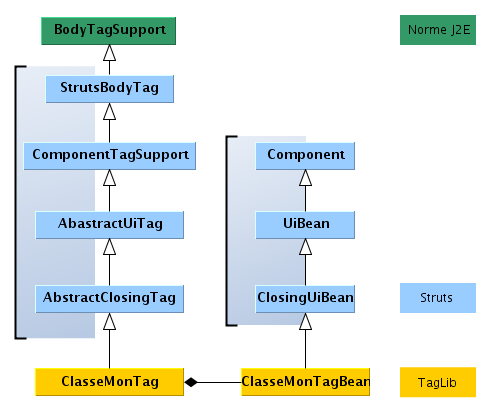
\includegraphics[height=7cm,width=9cm]{image/explicationTag.png}
  		\caption{Diagramme des tags avec struts}
  		\label{diagtagstruts}
\end{figure}

La création d'un tag classique, sans struts se fait par héritage de classe 
tel que "TagSupport" qui est une des classes définies dans la norme J2E pour la 
création des tags. En plus de la définition de la classe java, il faut écrire
dans un fichier xml (.tld) la définition du tag. La création de tag ainsi oblige
à écrire le code html directement dans le corps de la classe ou de devoir prévoir
l'architecture de support pour des templates.

Les templates permettent en fait de séparer le rendu du post-traitement effectué
sur les attributs d'un tag, il permettent aussi de supporter plusieurs "thèmes", 
c'est à dire des collections de css pour changer le rendu, etc.

Faire des tag comme struts c'est un peu différent donc, sur la figure \ref{diagtagstruts} 
on voit qu'il y a une certaine architecture déjà mise en place. Il y a une chaine 
d'héritage étendant la norme pour les tag, et de l'autre une chaine d'héritage 
de classe spécifique à struts. 

Pour créer des tags spécifiques on se place en bout de chaine, comme on le voit 
avec \emph{classeMontag} en héritant de \emph{AbstractClosingTag} on ne fait pas
grand chose, on délègue à la classe héritant de \emph{ClosingUiBean} qui contient 
elle la logique de traitement des éléments du tag. Ensuite il faut définir le
template écrit en \emph{freemarker}, qui lui contient le code html effectif 
qui sera écrit avec les éléments récupérés par la classe héritant de \emph{ClosingUiBean}.
Il faut aussi écrire le fichier tld pour la description.\\
\\
Pour résumer la création d'une taglib c'est:

\begin{itemize}
\item un fichier descripteur pour la taglib avec chaque tag de décrit 
\item une classe héritant de ClosingUiBean pour chaque tag
\item une classe héritant de AbstractClosingTag pour chaque tag qui délègue à son ClosingUiBean correspondant
\item des fichiers de template en freemarker pour chaque tag
\end{itemize}

Exemple de template freemarker:

\lstset{ %
language=HTML,                % the language of the code
basicstyle=\footnotesize,       % the size of the fonts that are used for the code               % where to put the line-numbers
  % the size of the fonts that are used for the line-numbers
                  % the step between two line-numbers. If it's 1, each line 
keywordstyle=\color[rgb]{0,0,1},
                      % will be numbered
numbersep=5pt,                  % how far the line-numbers are from the code
showspaces=false,               % show spaces adding particular underscores
showstringspaces=false,         % underline spaces within strings
showtabs=false,                 % show tabs within strings adding particular underscores
tabsize=2,                      % sets default tabsize to 2 spaces
captionpos=b,                   % sets the caption-position to bottom
breaklines=true,                % sets automatic line breaking
breakatwhitespace=false,        % sets if automatic breaks should only happen at whitespace
title=\lstname,                 % show the filename of files included with \lstinputlisting;
                                % also try caption instead of title
escapeinside={\%*}{*)},         % if you want to add a comment with
morekeywords={project,modelVersion,groupId,description,build, plugin,plugins,configuration, applicationName, wikittyServiceUrl, artifactId,serverID,uploadUrl} 
}



\begin{lstlisting}
<#include "/${parameters.templateDir}/${parameters.theme}/ws-label-commons.ftl" />
<select 
<#include "/${parameters.templateDir}/${parameters.theme}/ws-commons.ftl" />
 size="${parameters.selectSize}">
<#assign optionKeys = parameters.value/>
    <#list optionKeys as optionKey>
	<option value="${optionKey.valeur}"
	<#if  optionKey.valeur==parameters.value >
		selected
	</#if>
	> ${optionKey.description} </option>
	</#list>
</select>
\end{lstlisting}

Ce template, est le template pour le rendu en combobox ou liste de sélection,
il y a les éléments html et les éléments de langages freemarker. Avant que le
template soit remplit, les classes java correspondantes au tag remplissent 
un map de paramètres à laquelle a accès le template, d'où les structures de contrôle
pour itérer dans cette exemple. 


\subsection{La taglib wikitty struts "ws"}

Les tags ainsi développés ont deux utilisations possibles, la création d'un 
formulaire d'édition de wikitty, ou la création de formulaire utilisant les 
champs de wikitty comme champs. 

La différenciation de l'utilisation des tags passent par l'utilisation du tag 
de la taglib ws:form, qui implique que dans ce cas on se trouve dans l'édition d'un
wikitty.

A l'utilisation si on met seulement le tag \emph{ws:form} et la source de donnée 
(le wikitty) un formulaire basique va être créé en fonction du type des champs
du wikitty. Ensuite en utilisant les autres tags ou différents attributs du tag 
\emph{ws:form} il est possible de choisir d'exclure de l'édition des extensions,
des champs ou de choisir le type d'affichage pour un champ donné (et identifié
par son nom complet soit nomExtention.nomChamp).

En plus de fournir des tags pour la création de formulaire, la tag lib propose 
une action qui permet de prendre en compte les modifications de wikitty envoyées
par le formulaire. Il s'agit d'une action abstraite struts que l'utilisateur à 
besoin d'étendre pour implémenter la méthode accédant au proxy.

Tags commun aux deux types d'utilisations:
\begin{itemize}
\item ws:hidden permet d'insérer le champ en tant que champs caché
\item ws:boolean permet d'insérer le champ en tant que checkbox 
\item ws:textArea permet d'insérer le champ en tant que textArea
\item ws:textField permet d'insérer le champ en tant que textField
\item ws:date permet d'avoir un composant intelligent pour les dates 
\item ws:selectFixed permet d'afficher un combobox avec des valeurs fixées à 
l'avance, sera sélectionnée celle correspondant au champs wikitty liés
\item ws:selectCriteria permet d'afficher un combox box avec des wikitty, 
sera sélectionnée le wikitty correspondant à l'id du wikitty du champ
(utilisé donc dans le cadre de relation entre wikitty)\\
\end{itemize}

Tag spécifique pour la création de formulaire:
\begin{itemize}
\item ws:form tag pour la création d'un formulaire d'édition des wikitty \\
\end{itemize}

Tags spécifiques à l'utilisation champ:
\begin{itemize}
\item ws:selectAssociation tag pour l'affichage de champ wikitty de type collection
\item ws:select tag pour l'affichage de collection de wikitty en tant que list ou combobox html
\end{itemize}



